\clearpage\section{Data model and schema mapping}\label{sec:data}
\subsection{Conceptual model}
The model covers GENAILMS's own PostgreSQL schema; Moodle is external, and the Moodle course, user and activity ids stored here are references to it. Figure~\ref{fig:erd-overview} shows all entities and cardinalities in Chen notation; the attributes are given in the mapping tables. A course contains documents; a document has chunks and produces modules; a module has components, and question-bearing components have questions. The research and operational entities are listed in Table~\ref{tab:05-data-2}.
\begin{landscape}
\thispagestyle{plain}
\begin{figure}[H]\centering
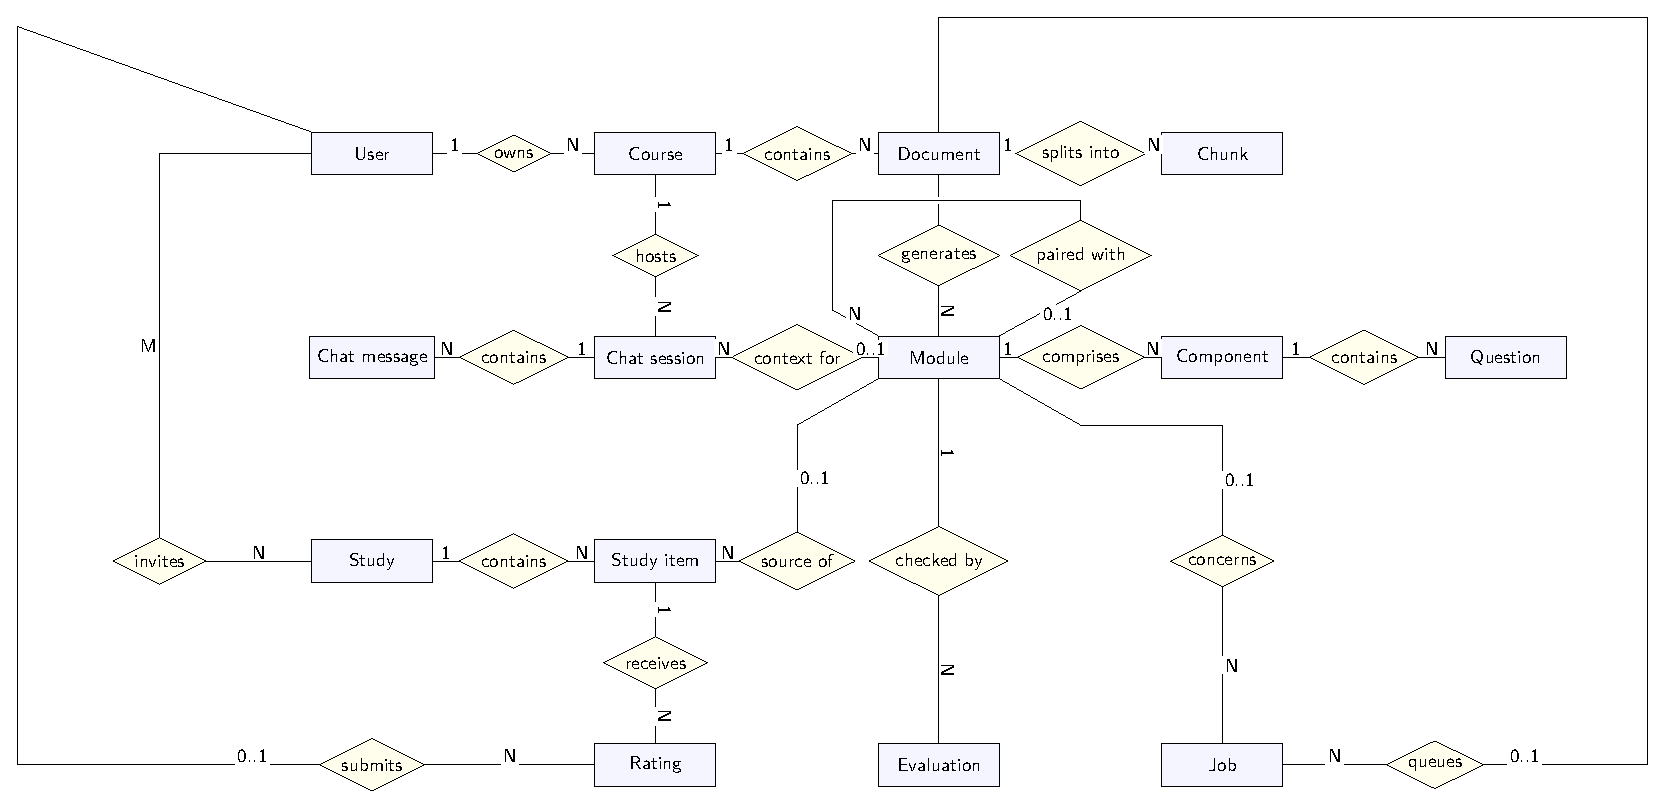
\includegraphics[width=\linewidth,height=.82\textheight,keepaspectratio]{diagrams/erd-overview.pdf}
\caption{Complete Chen overview: entities and relationships without attributes. M and N denote independently varying many sides (including zero); 1 denotes exactly one; 0..1 denotes an optional single entity.}
\label{fig:erd-overview}
\end{figure}
\end{landscape}
\needspace{10\baselineskip}
\subsection{Core relational mapping}
\begin{longtable}{|p{2.8cm}|p{7.0cm}|p{4.1cm}|}\caption{Core entity-to-table mapping.}\label{tab:schema}\\\hline
Table & Important columns and keys & Purpose / invariant\\\hline\endfirsthead
\hline Table & Important columns and keys & Purpose / invariant\\\hline\endhead
\code{users} & universally unique identifier (UUID) primary key (PK); unique email; password hash; active/admin/can-author flags; optional unique Moodle user ID; model preference; daily chat count & Local identity independent of Moodle confirmation\\\hline
\code{courses} & UUID PK; owner foreign key (FK) to users; name; nullable Moodle course ID & Owned authoring workspace; remote target may be shared by multiple app courses\\\hline
\code{course_members} & Composite PK (course, user); source & Read-only access for LTI learners (Section~\ref{sec:lti-learners})\\\hline
\code{documents} & UUID PK; course FK; filename; status; raw text; planner cache & Document processing and concept planning\\\hline
\code{chunks} & UUID PK; document/course FKs; ordered chunk index; content; source reference; vector(768) & Evidence unit and retrievable passage\\\hline
\code{modules} & UUID PK; document/course FKs; title; LO; Bloom level; sub-objectives; generation payload/models; optional paired-module FK & Saved module and experimental pairing\\\hline
\code{module_components} & UUID PK; module FK; type; JSONB content; unique (module, type) & One row per non-LO component type\\\hline
\code{questions} & UUID PK; component FK; stem; choices JSONB; answer key; explanation; position & Editable and exportable quiz/practice questions\\\hline\end{longtable}
The LO fields belong to \code{modules}, so the seven parts are six component types plus those fields. Component content is JSONB. The \code{course_id} copied onto chunks and modules makes course filters and row-level security cheap; a composite foreign key to \code{documents(id, course_id)} prevents such a row from naming a different course from its document. A unique (module, type) pair prevents two Content rows in one module, and explicit positions order chunks and questions.
\subsection{Operational and research mapping}
\begin{longtable}{|p{3.0cm}|p{6.6cm}|p{4.3cm}|}\caption{Operational and research entities.}\label{tab:05-data-2}\\\hline
Table & Key fields and links & Behavior\\\hline\endfirsthead
\hline Table & Key fields and links & Behavior\\\hline\endhead
\code{jobs} & Type, document/module references, step, status, payload, attempts, due time, lock metadata, last error and whether the system caused a failure & PostgreSQL-backed processing queue; nullable links depend on job type\\\hline
\code{evaluations} & Module FK, criterion, numeric score and notes & Pipeline checks; not formal blind ratings\\\hline
\code{chat_sessions} & Course FK, user FK and optional module FK & Course Q\&A or module-specific editing context; visible only to its user\\\hline
\code{chat_messages} & Session FK, role, text, citations and applied-edit flag & Persisted conversation and edit evidence\\\hline
\code{refresh_tokens} & User FK, unique token hash, expiry and revocation & Server-side session renewal control\\\hline
\code{studies} & Name, rubric version, status and JSONB invited email list & Draft/active/closed study organization\\\hline
\code{study_items} & Study FK, anonymous code, group, nullable source module FK and JSONB packet & Frozen blinded material; group hidden from raters\\\hline
\code{ratings} & Item FK, nullable user FK, rater kind, eight score/reason objects and notes & Human rating or LLM-judge slot, separate from pipeline checks\\\hline
\code{lti_platforms}, \code{lti_deployments} & Issuer, client id, key-set and token URLs; registered deployments & Platforms allowed to launch the tool\\\hline
\code{lti_identities}, \code{lti_contexts} & (platform, \code{sub}) to user; (platform, deployment, context) to course; roster address and last check & Who a launch is and which course it opens\\\hline
\code{lti_login_states}, \code{lti_launch_codes} & State and nonce with a 10-minute expiry; one-time launch code & Single use; kept in PostgreSQL so any task can finish a launch\\\hline\end{longtable}
A study item is a frozen packet; a RAG item also references its module, while the no-RAG item of a pair is self-contained. Ratings hold one row per human rater and item, and one per judge family and item. Foreign keys from studies use \code{RESTRICT}, so a module used in a study cannot be deleted silently; the API answers 409 instead.
\subsection{Citation and edit representation}
The server stores a \code{source_map} from codes such as S1 to a chunk id and its locator, and derives \code{inline_citations} from the saved Markdown with the character offsets of each claim and marker. Unknown codes are rejected. On the first edit, an \code{ai_original} object in the component keeps the version before editing, including the ordered questions and explanations; later edits do not change it.
